\begin{figure*}[hbtp]
  \centering
  % \includegraphics[width=0.44\linewidth]{out/5050-runtime-key.pdf}
  \subfigure[Overall result]{
    \label{fig:5050-runtime--mean}
    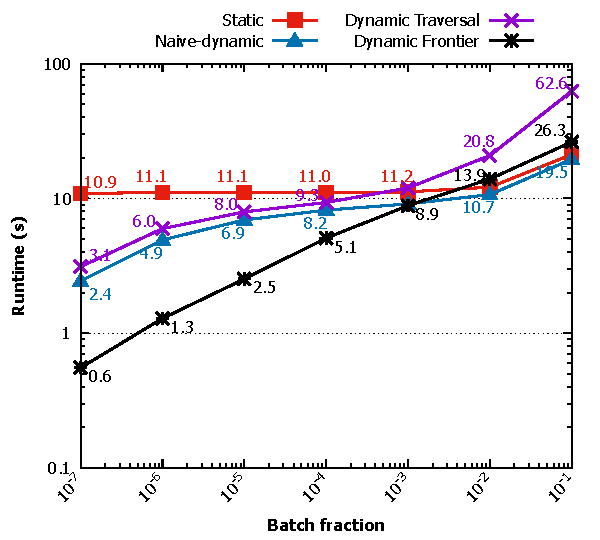
\includegraphics[width=0.38\linewidth]{out/5050-runtime-mean.pdf}
  }
  \subfigure[Results on each graph]{
    \label{fig:5050-runtime--all}
    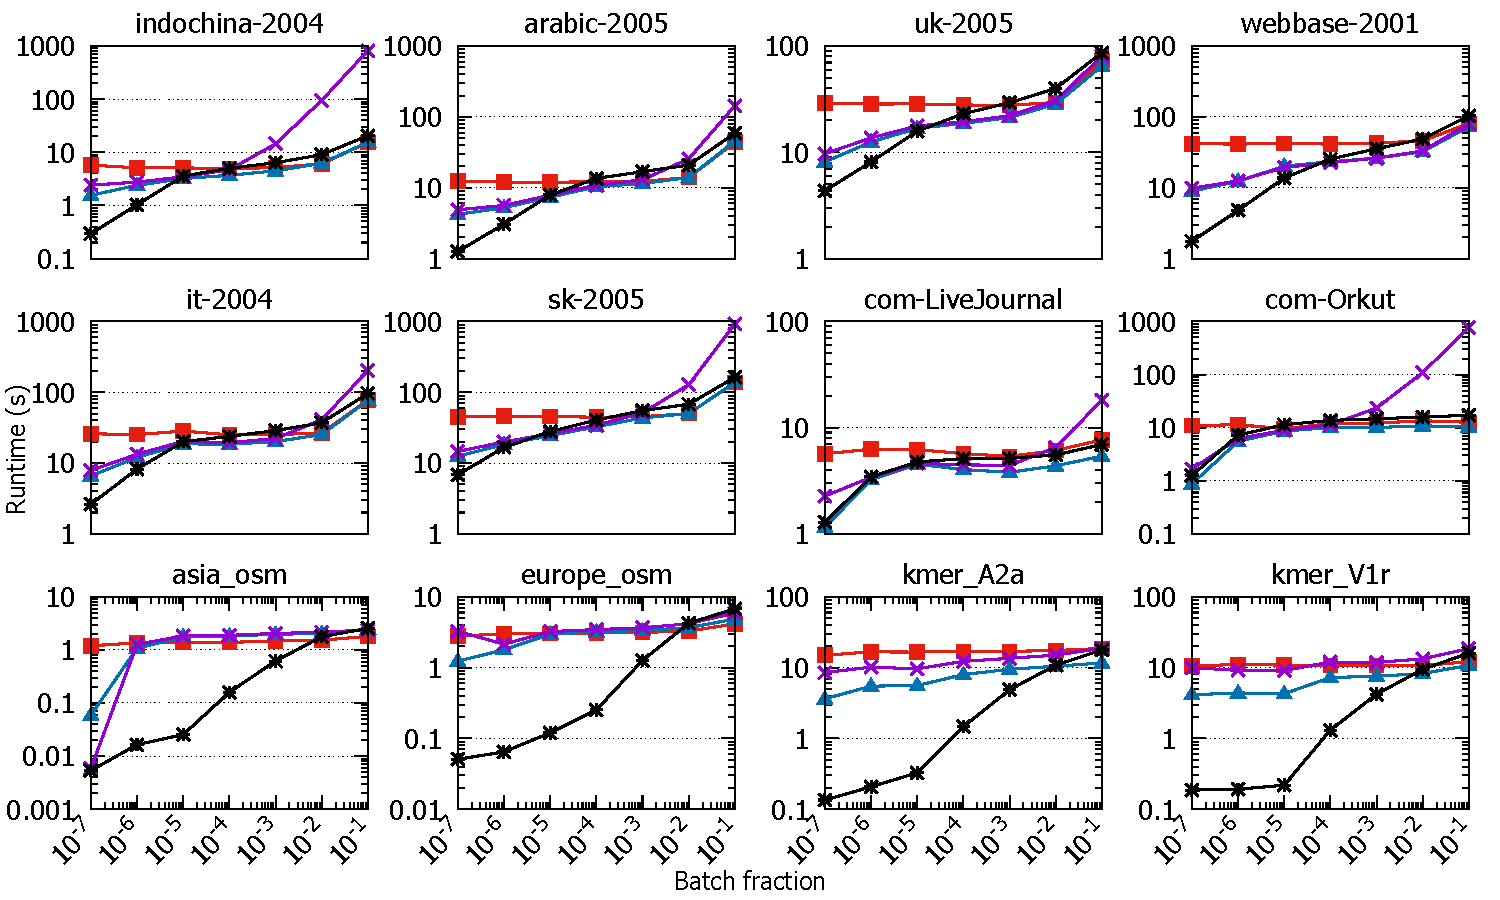
\includegraphics[width=0.58\linewidth]{out/5050-runtime-all.pdf}
  } \\[-1ex]
  \caption{Runtime (logarithmic scale) of \textit{Static}, \textit{Naive-dynamic}, \textit{Dynamic Traversal}, and \textit{Dynamic Frontier} PageRank with batch updates increasing from $10^{-7} |E|$ to $0.1 |E|$, in multiples of $10$ (logarithmic scale). The updates include $80\%$ edge insertions and $20\%$ edge deletions, simulating realistic changes upon a dynamic graph. The figure on the right illustrates the runtime of each approach for each graph in the dataset, while the figure of the left presents overall runtimes (using geometric mean for consistent scaling across graphs).}
  \label{fig:5050-runtime}
\end{figure*}
